\section{Introduction}
\label{sec:intro}

Covalent organic frameworks (COFs) entered materials chemistry in 2005, when boronate-ester
condensation delivered the first crystalline, porous, fully organic frameworks with pore sizes
of 7--27~\AA{} and high thermal stability~\cite{cote2005porous}. Photocatalysis arrived nine
years later: a hydrazone-linked TFPT-COF bearing 3.8~nm mesopores produced hydrogen from water
under visible light with a Pt cocatalyst, establishing COFs as a designable photocatalyst
class~\cite{stegbauer2014a}. The decade since has been
one of rapid quantitative progress: linkage-protonated donor--acceptor (D--A) COFs now reach
hydrogen evolution rates of 20.7~mmol\,g$^{-1}$\,h$^{-1}$~\cite{yang2021protonated}, D--A COF
nanosheets report apparent quantum efficiencies (AQE) of 82.6\% at
450~nm~\cite{li2022covalent}, and framework reconstruction strategies push sacrificial rates to
27.98~mmol\,h$^{-1}$\,g$^{-1}$~\cite{zhang2022reconstructed}.

Existing reviews organize this literature primarily by material family or application
class~\cite{wang2020covalent,chen2024photocatalysis}. That organization answers ``which COF has
been made,'' but not the question a synthetic chemist actually faces: \emph{which design lever
moved the number, and what should I therefore synthesize next?} Mechanistic perspectives have
begun to frame COF photocatalysis as a pipeline --- photon absorption, exciton dissociation,
charge transport, and interfacial reduction --- whose weakest stage caps the overall
rate~\cite{blatte2024photons}. This survey adopts that pipeline view and contributes:

\begin{itemize}
\item \textbf{C1 --- A factor-chain taxonomy} (Fig.~\ref{fig:factorchain}). Five lever groups
  --- linkage chemistry (L1), band-structure engineering (L2), exciton and crystallinity
  management (L3), interfacial catalysis (L4), and synthesis methodology (L5) --- are mapped
  onto the pipeline stage each principally governs, with at least three primary references per
  taxonomy leaf (Secs.~\ref{sec:levers}--\ref{sec:synthesis}).
\item \textbf{C2 --- An evidence-chained gap register.} Six research gaps, each grounded in at
  least two audited library references with database provenance and explicit reasoning about
  why current work leaves the gap open (Sec.~\ref{sec:challenges}).
\item \textbf{C3 --- A survey-to-synthesis bridge.} A decision-recorded synthesis and
  process-optimization plan for the $\beta$-ketoenamine COF TpPa-1, converting the factor-chain
  evidence into an executable, safety-annotated protocol with a quantified route comparison and
  a thermodynamic feasibility audit (Sec.~\ref{sec:routec}).
\end{itemize}

\begin{figure}[t]
  \centering
  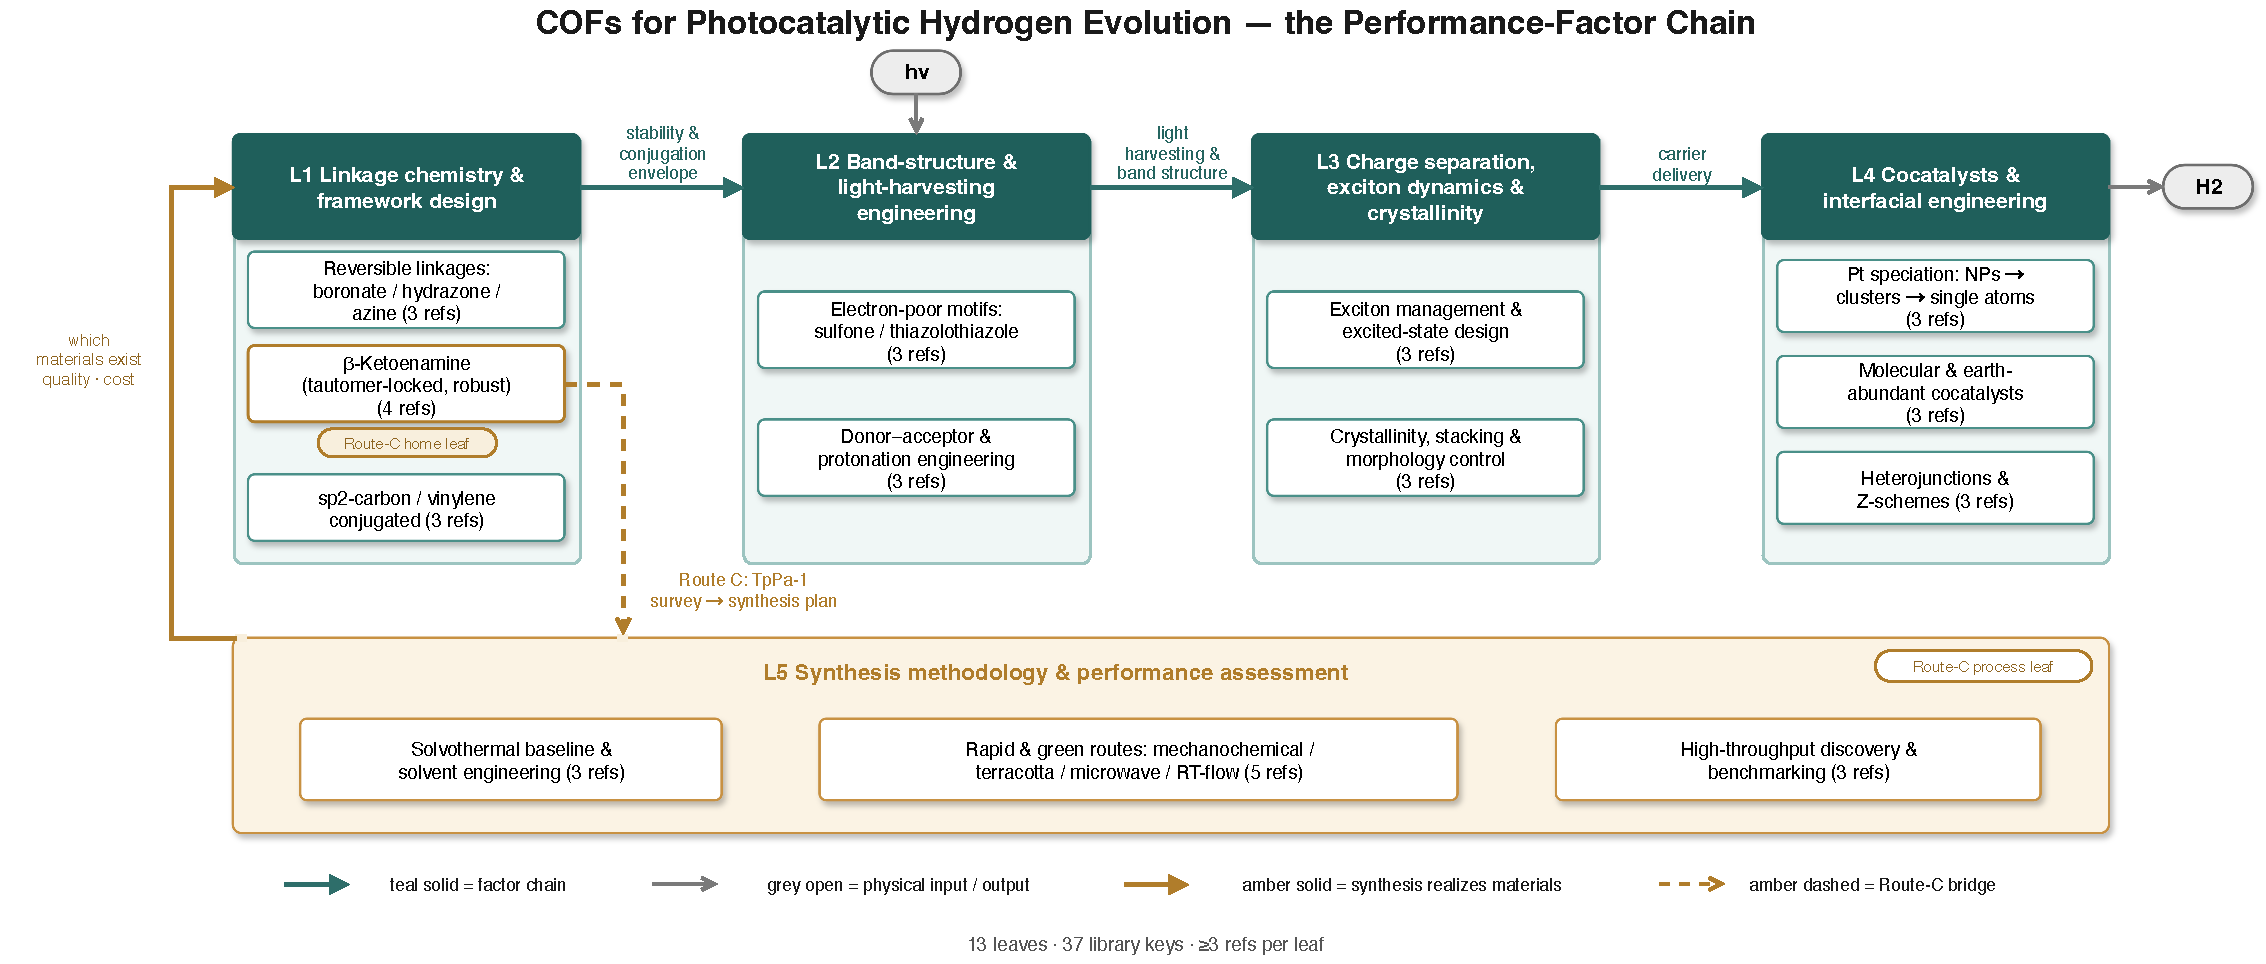
\includegraphics[width=\linewidth]{figures/fig1_factor_chain.pdf}
  \caption{Factor-chain taxonomy of COF photocatalysts for the hydrogen evolution reaction
  (HER). Top: five groups of design levers (L1--L5) identified in this survey; bottom: the
  photon-to-H$_2$ physical pipeline. Labeled arrows mark the pipeline stage each lever family
  principally governs; the synthesis level (L5) acts indirectly by setting crystallinity and
  phase purity.}
  \label{fig:factorchain}
\end{figure}

Scope follows the audited protocol of this project: crystalline 2D/3D COFs evaluated for
sacrificial photocatalytic HER, plus synthesis-methodology studies of the TpPa family required
by C3; metal--organic frameworks, CO$_2$ photoreduction, and pure oxygen-evolution studies are
excluded. All 37 cited references were retrieved by multi-source search (arXiv, OpenAlex,
Crossref) and passed a zero-tolerance citation-integrity audit; the audit trail is part of the
deliverable. The survey is written for materials and chemistry graduate students: the intended
takeaway is a mental model of \emph{which factor limits which performance regime}, plus a
reusable template for turning literature evidence into a synthesis decision.
